\subsection{The Need for a New OS Framework}
\label{emt:sec:need}

\begin{figure}[H]
	\centering
\begin{minted}[xleftmargin=17.5pt,linenos,breaklines,fontsize=\small,escapeinside=@@]{C}
void vunmap_pmd_range(pmd, addr, end) {
  @\codetype{pmd\_t}@ *pmd = @\codehl{pmdoff}{pmd\_off}{set(pud}@, addr);
  do { ...
    // try remove huge page entry
    int cleared = pmd_clear_huge(pmd);
    ...
    if (@\codehl{pmdnone}{pmd\_none\_}{or\_clear\_bad}@(pmd))
      continue;

    // try remove underlying PTEs
    vunmap_pte_range(pmd, addr, next, mask);
    ...
  }
  while (@\codehl{pmdpp}{pmd}{++}@, addr = next, addr != end);
} /* mm/vmalloc.c */
\end{minted}
\caption{\bf Examples of Linux memory management code that is hardwired to
radix-tree based translation.} 
% \jyk{As a reviewer, I am curious how this code example
% has been changed with \branding. How about showing the EMT version too, explaining
% how we addressed each memory semantic overload.}}
\label{emt:fig:need:linux-no-interface}
\end{figure}

\noindent
Emerging memory technologies and research on MMU architectures
	pose a strong need 
	of %an effective OS framework
	%for 
	developing and evaluating OS memory management 
	on new translation schemes.
The current practice of evaluating new translation schemes mostly relies on hardware simulation, 
	either using performance models to estimate OS overhead~\cite{self:dmt,margaritov2019asap,yaniv2016hash,karakostas2015redundant,alverti2020enhancing,ryoo2017rethinking},
	or replaying traces
	collected by running workloads on vanilla Linux~\cite{skarlatos2020ecpt,ryoo2017rethinking,yaniv2016hash,margaritov2019asap}.
% However, translation architectures
%	could have a significant impact on OS performance,
%	which is hard to understand or model. % without developing the OS componnet.
Such approaches can hardly capture complex OS-architecture interactions~\cite{anderson91mach}.
We argue that the lack of OS effort is largely due to memory management systems 
	in commodity OSes not providing an extensible interface for new, different translation architectures.

% We argue that major OSes today lack support for developing and experimenting with
%	OS memory management on new memory translation architectures.

% With the scale of memory capability, 
    % not only elevate off-TLB translation overhead
	% into a pressing issue, but also changes 
%	the design tradeoff of translation architectures---new 
% ---space-efficiency of in-memory translation structures
%	is no longer the foremost requirement, compared to translation speed.
%	architectures no longer optimize space-efficiency but focus on speed,
%	
%	or by shortening trees~\cite{park2022fpt}.
% Memory heterogeneity (e.g., \TODO{enabled by CXL.mem~\cite{}})
%	and diverse computing patterns (long-running memory-intensive workloads verus short-lived serverless functions)
%	indicates versatile, hybrid translation schemes.

% \vspace{-5pt}
% \subsubsection{Hardwiring Translation Schemes is Untenable}
% \label{emt:sec:need:hardwire}

\para{Hardwiring Translation Schemes Is Untenable.}
\noindent
Linux's memory management code is currently hardwired to a five-level tree.
Without an extensible framework,
	it can hardly embrace new translation architectures that use 
	different lookup structures such as hash tables~\cite{skarlatos2020ecpt,yaniv2016hash,jovan2023memory}, 
	flattened or range tables~\cite{park2022fpt,karakostas2015redundant,ahn2012revisiting}, 
	and hybrid schemes~\cite{kanellopoulos2023utopia,alam2017doityourself}.

% \begin{figure}
% 	\centering
% 	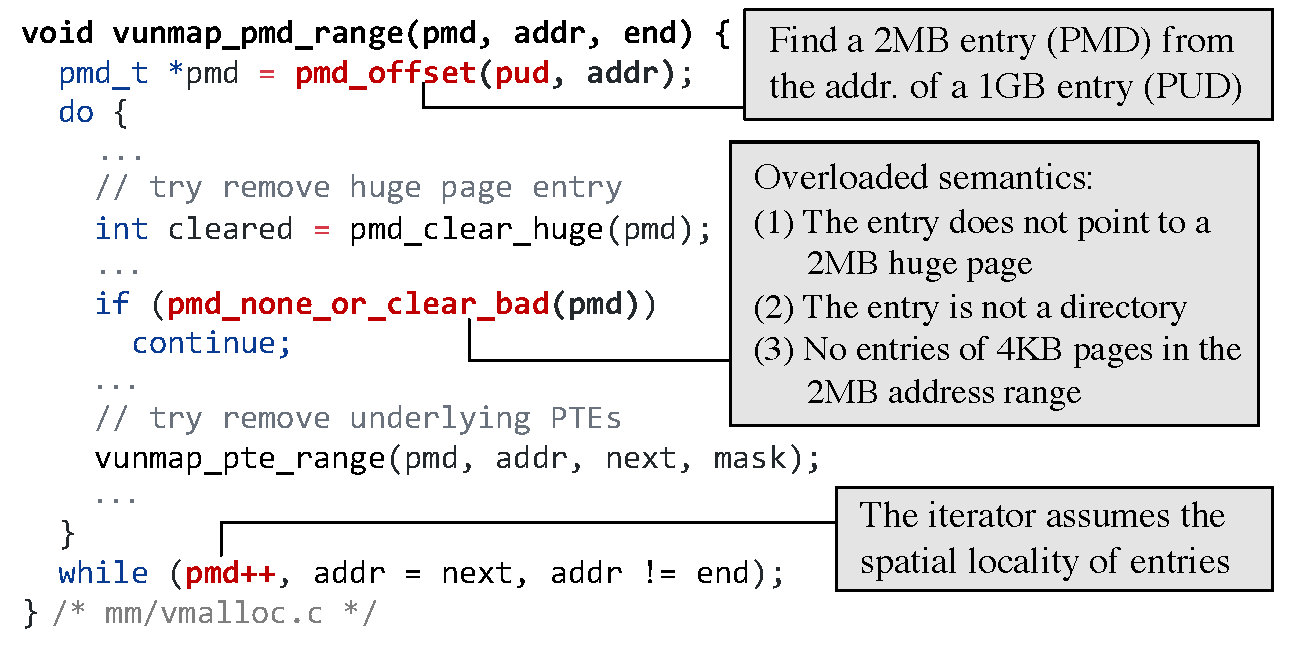
\includegraphics[width=0.49\textwidth]{figs/linux-no-interface}
% 	\vspace{-25pt}
% 	\caption{\bf Examples of Linux memory management code that is hardwired to
% 	tree-based translation.}
% 	\label{emt:fig:need:linux-no-interface}
% 	\vspace{-12.5pt}
% \end{figure}



Figure~\ref{emt:fig:need:linux-no-interface} shows a representative example in Linux, where a memory
	operation for unmapping a virtual address range at PMD level (\texttt{\small vunmap\_pmd\_range} in \texttt{\small vmalloc.c}) 
	makes the following
	assumptions specific to Linux's tree definition:
\begin{packed_itemize}%[\labelitemi]
		\item A translation entry of a 2MB virtual address range (PMD)
			can be found from the entry of a 1GB address range.
		\item An entry of a 2MB address range (PMD) either points to 
			a 2MB huge page or a directory of 4KB pages.
		\item The translation entry of the next 2MB address range can be 
			iterated by increasing the pointer.
\end{packed_itemize}
% None of these assumptions hold true for hashing-based translation.
Such implementation patterns are commonplace in Linux's current architecture-independent memory management module.
Hence, supporting a different translation architecture would require heavy rewriting
	of existing Linux code.

In fact, 
	it is \schai{also} nontrivial for Linux to support translation schemes that use a different tree. %(e.g., a short tree~\cite{ahn2012revisiting,park2022fpt})
%	without substantial code changes. % due to the hardwired 5-level tree.
Evidently, adding the fifth level took 715 lines of code changes across 23 files~\cite{linux:5levelimpl},
	all in the architecture-independent modules of Linux.
Similarly, though FPT's design strives to limit OS changes~\cite{park2022fpt},
	it still introduces nontrivial changes of Linux's architecture-independent code
	to fold the intermediate levels of the tree.
	
% For example, to support Intel's new five-level page table, Linux had to upgrade its translation abstraction from four to five levels,
%	a process that required modifying dozens of architecture-independent code files, leading to a switch cost and long adoption latency.

Furthermore, without a well-defined interface, memory management code becomes hard to maintain
	due to implicit assumptions and semantic overloads with continuous optimizations and fixes.
In Figure~\ref{emt:fig:need:linux-no-interface}, \texttt{\small pmd\_none\_or\_clear\_bad()} 
	overloads three semantics, making the code hard to maintain.

%	as Linux is the dominating OS kernel for high-performance, memory-intensive computing,
%	the lack of extensibility has become a barrier to hardware innovations as discussed in \S\ref{emt:sec:intro}.
% because it is a must to have kernel support for new hardware
%	for evaluation;
%	simulation helps, but is insuffient as we will show in our evaluation.

\begin{comment}
\begin{figure}[H]
	\centering

	\begin{minted}[xleftmargin=20pt,linenos,mathescape,breaklines,fontsize=\small]{C}
struct file_operations {
  ssize_t (*read) (struct file *, char __user *, size_t, loff_t *);
  ssize_t (*write) (struct file *, const char __user *, size_t, loff_t *);
  loff_t (*llseek) (struct file *, loff_t, int);
  int (*iterate) (struct file *, struct dir_context *);
  // ...
};
\end{minted}

	\caption{Part of the VFS interfaces.
		VFS assumes the presence of a directory tree and everything is a variable-length file.
		Such assumptions are not held for page-based address translation,
			leading to both redundancy and deficiency when serving as an address translation interface.}
\label{emt:code:vfs}
\end{figure}
\end{comment}

\begin{figure}[H]
	\centering
\begin{minted}[xleftmargin=17.5pt,linenos,mathescape,breaklines,fontsize=\small,escapeinside=@@]{C}
void walk_pte_range(pmd, addr, end, walk) {
  @\codetype{spinlock\_t}@ *ptl;
  @\codetype{pte\_t}@ *pte = @\codehl{linuxlock}{pte\_offset}{\_map\_lock}@(mm, pmd, addr, &ptl);
  ...
  for (;;) {
    err = ops->@\codehl{linuxpte}{pte\_e}{ntry}@(pte, addr, addr + PAGE_SIZE, walk);
    ...
    addr += PAGE_SIZE;
    @\codehl{linuxiter}{pte}{++;}@
  }
  ...
  pte_unmap_unlock(pte, ptl);
} /* mm/pagewalk.c */
\end{minted}

\caption{\bf Hardware-specific optimizations in Linux.}
\label{emt:fig:need:linux-performance-opt}
\end{figure}

% \begin{figure}
% 	\centering
% 	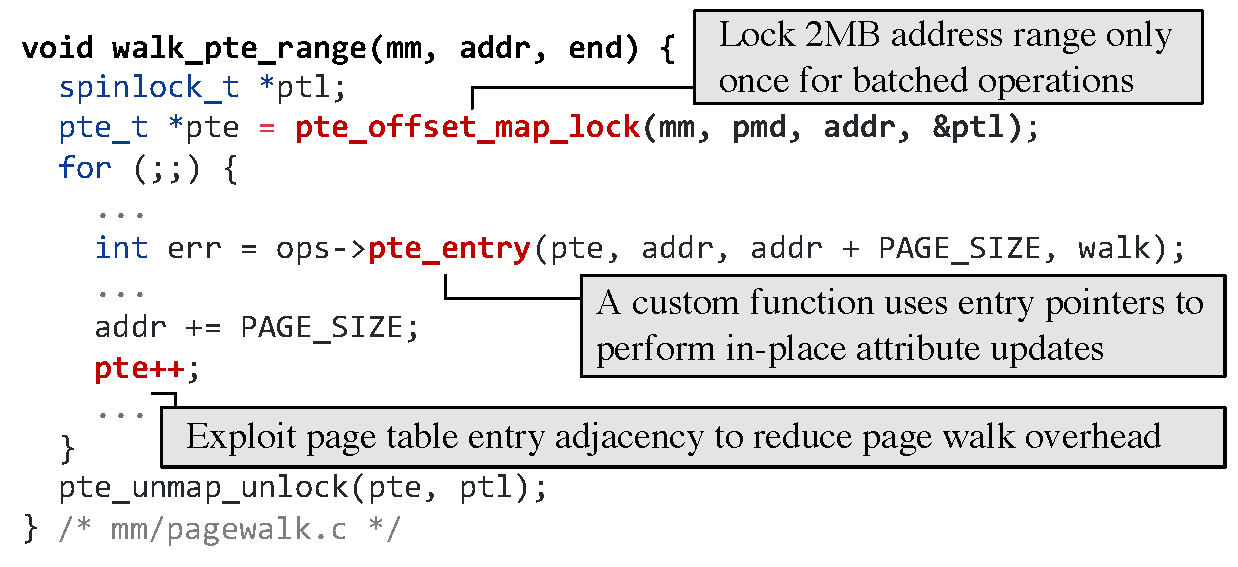
\includegraphics[width=0.49\textwidth]{figs/linux-performance-opti}
% 	\vspace{-25pt}
% 	\caption{\bf Hardware-specific optimizations in Linux.}
% 	\label{emt:fig:need:linux-performance-opt}
% 	\vspace{-12.5pt}
% \end{figure}

\para{Hardware-Specific Optimizations Are Desired.}
%\label{emt:sec:need:llopt}
Inspired by Mach/BSD~\cite{freebsd:pmap,cranor99uvm,rashid1987machine} 
	that have clean separation of machine-independent and dependent code,
	we started from a pmap-like interface for Linux.
% The related interface in BSD/Mach is pmap
% that separate machine independent and dependent modules.
\schai{In Mach/BSD, architecture-indepedent memory management code uses pmap interface to 
	manage virtual memory mappings.}
pmap~\cite{rashid1987machine} represents a \schai{virtual-to-physical} 
	address map, which 
% can be implemented based on hardware MMU---a pmap 
	can point to a VAX linear page table~\cite{levy82virtual} 
	or segment registers in IBM RT PC.
With pmap, different translation schemes can be supported
	by writing %corresponding 
	pmap modules.
\schai{Typical pmap operations include 
	creation, deletion, and update of address mappings~\cite{rashid1987machine,freebsd:pmap}.}
% Similar map interfaces are used in early OSes like SunOS~\cite{gingell1987sunos}.
% \TODO{perhaps mention GMI and SunOS have a similar interface.}

Unfortunately, we find that a map interface like pmap is not
	sufficiently expressive to write hardware-specific optimizations,
	especially in the Linux context. %, without introducing new abstractions (e.g., page and memory objects in Mach/BSD).
For example, pmap routines % like \texttt{\small pmap\_enter()} and \texttt{\small pmap\_extract()},
	for inserting or finding a translation, 
	only reference a virtual address without exposing
	translation entries.
% The interface makes low-level optimizations hard. 
Figure~\ref{emt:fig:need:linux-performance-opt} shows three common patterns of optimizations in existing Linux code:
	1) batching with fine-grained locks for range operations,
	2) in-place translation entry updates with no data copy,
	and 3) direct fetching of translation entries by offsets. 
None of them are easy to write using a map,
	as they need to directly manipulate translation entries.
% \weiwei{TODO: think about how to clearly let people understand why these three examples
% expose low level optimizations; now, it is unclear to me. My suggestion is that we may
% use a comparison approach: without/with low level optimizations, what things will look like.}
As optimizations of memory management are critical to Linux performance---27.8\%
	of Linux kernel patches to memory management are for performance optimizations~\cite{huang16mmstudy}---a
	simple map interface makes it hard to fully empower translation architectures.
% A challenge of extensibility and inclusivenessis to 
%	avoid impairing Linux performance.
	
%	being extensible to generalizability and specialization. 

% \subsubsection{Summary}

% From the hardware architecture research standpoint,
%	% as Linux is a dominating OS for memory-intensive datacenter computing,
%	the lack of extensibility of memory management system with regards to translation architectures
%	has become a major barrier to understanding new architecture designs and evaluating them.
% Hardware simulation helps but is hard to reflect the OS perspective, which is critical to system performance.
% implications on
%	OS memory management, 
% As translation architectures have been a main focus of innovations,
%	we advocate for an extensible OS framework to embrace new translation
%	architecture designs and to prevent a forced inclination to an incremental research agenda.

% However, for new paging-based novel address translation designs,
%	this design reduces the visibility of low-level yet architecture-neutral details\footnote{Such as the location/pointer of a PTE.},
%	prevents optimizations that rely on such intermediate results,
%	and results in a loss of performance and scalability.
%
% For example, both  of the Mach interface use only virtual addresses as the reference.
% This forces each insert and query operation to traverse the entire page table hierarchies or perform a full hash table lookup,
%	which has a negative performance impact on such operations when multiple neighboring pages are involved.
%

% (tianyin) this point is untrue as it can be done by creating common utils
% Moreover, to enforce virtual address-level encapsulation,
%	all address space operations must be done inside the architecture-dependent code,
%		even some mundane ones like \texttt{pmap\_copy\_page} and \texttt{pmap\_zero\_page}.
% For the increasingly complex modern memory management subsystem,
%	this design compromises scalability and prevents the reuse of potential architecture-neutral codes across architectures.


\begin{comment}
\begin{figure}[H]
	\centering
\begin{minted}[xleftmargin=20pt,linenos,mathescape,breaklines,fontsize=\small]{C}
int pmap_enter(pmap_t pmap, vm_offset_t va, vm_page_t m, vm_prot_t prot, u_int flags, int8_t psind);
vm_paddr_t pmap_extract(pmap_t pmap, vm_offset_t va);
void pmap_copy_page(vm_page_t, vm_page_t);
void pmap_zero_page(vm_page_t);
// ...
\end{minted}

	\caption{Part of the FreeBSD-optimized Mach interface.
		Mach uses virtual addresses as the reference and pushes certain operations to architecture-dependent parts,
			resulting in a loss of performance and scalability.}
\label{emt:code:bsd}
\end{figure}
\end{comment}

%%%%%%%%%%%%%%%%%%%%%%%%%%%%%%%%%%%%%%%%%%%%%%%%%%%%%%%%%%%%%%%%%%%%%%%%%%%

\para{Existing Frameworks Do Not Target Translation.}
Driven by new memory technologies like tiered memory, 
	several new memory management frameworks~\cite{Tabatabai2024,Raybuck2021,Jalalian2024}
	have been developed to improve the extensibility of Linux's memory manager.
However, few of them concern hardware translation architectures,
	but focus on application-specific page prefetching and replacement policies.
% To improve the extensibility of memory management in Linux,
%	recent work proposes File-Based Memory Management (FBMM).
FBMM~\cite{Tabatabai2024} proposes to 
	reuse VFS~\cite{linux:vfs} and write memory managers as file systems.
It exposes the \texttt{\small page\_fault} VFS callback for managing page table entries.
% The idea is to 
% Specifically, VFS exposes routines 
%	for memory-mapped files to manage translations.
% FBMM provides a way to improve extensibility of Linux memory management, 
%	enabling features such as memory tiering.
% However, FBMM mostly focuses on memory tiering and does not address 
%	translation architectures: 
However, FBMM relies on 
	Linux's existing code that is hardwired 
	to the multi-level radix tree structure,
	and thus cannot support different hardware translation schemes.
Fundamentally, file system interfaces can hardly serve as an effective 
	framework for memory translation.
% native support for %for variable-length files with directory hierarchy
%	memory management. % especially low-level translation.
%	is not native to fixed-length pages with flat address space.
% Moreover, it is hard for FBMM to achieve high performance due to the semantic mismatch.
% For example, with 4KB pages, FBMM is 50\% slower than vanilla Linux
%	due to the overhead in ext4 DAX of allocating pages, 
%	an artifact of the VFS design for file workloads instead of memory management~\cite{tabatabai2023fbmm}.
% (we didn't evaluate on new memory devices so let's be safe as the argument on FBMM is sufficient)
% \weiwei{Prior works~\cite{alverti2022daxvm,papagiannis2020optimizing} also show that
%	memory-mapped files show significant overhead while using new memory devices.}

%One of the state-of-the-art generic interface designs in Linux is the file-system-oriented VFS interface.
% FBMM~\cite{} has proposed to reuse VFS as an extensible interface for kernel memory management.
% However, this approach has several drawbacks in the realm of address translation.
%
% First, the abstraction VFS employs is variable-length files with directory hierarchy.
% However, this design can be redundant for address translation that works with fixed-length pages and flat address spaces.
%
% Second, VFS lacks specific interfaces to accomplish necessary architectural operations while others are redundant.
% For example, both page tables and PTE are frequently read and written,
%	whereas, under the VFS interface (Figure \ref{emt:code:vfs}), there is only a single (\texttt{file}-based) \texttt{read}/\texttt{write} interface.
% This forces an semantic overlap between PT operations and PTE operations.
% Yet, VFS provides interfaces like \texttt{llseek} and \texttt{iterate} that are not needed by address translation.
%
% And, finally, it has been evaluated~\cite{} that when used for memory management, VFS has a performance overhead of up to 50\%,
%	which is untenable for modern address translation that already bears high overhead.